
\chapter{变换矩阵}
\label{chap07}

线性代数可以用来表达许多操作,包括在三维场景中排列物体、用摄像机查看物体,以及将场景投影到屏幕上。旋转、平移、缩放和投影等几何变换可以用矩阵乘法来完成,本章的主题就是可以完成这些变换的矩阵。

如果一个点集被表示为从原点出发的偏移向量,我们将展示这些点是如何转换的,我们将用图\ref{fig:7.1}中的时钟作为一个点集的例子。因此,可以把时钟看成是一群点,它们是尾部在原点的向量的两端。我们还讨论了这些变换对位置(点)、位移向量和表面法向量的不同操作。

\section{二维线性变换(2D Linear Transformations)}

我们可以使用一个$2 \times 2$的矩阵来改变或者变换一个二维向量:

\begin{equation}
	\left[\begin{array}{ll}
		a_{11} & a_{12} \\
		a_{21} & a_{22}
	\end{array}\right]\left[\begin{array}{l}
		x \\
		y
	\end{array}\right]=\left[\begin{array}{l}
		a_{11} x+a_{12} y \\
		a_{21} x+a_{22} y
	\end{array}\right]
\nonumber
\end{equation}

这种通过简单矩阵乘法将一个二维向量与另一个二维向量相乘的操作,称为线性变换。通过这个简单的公式,我们可以实现各种有用的转换,这取决于我们在矩阵中放置的内容,这将在下面的章节中讨论。为了方便,考虑沿x轴移动是水平移动,沿y轴移动是垂直移动。

\subsection{缩放(Scaling)}

最基本的变换是沿坐标轴的缩放。该变换可以改变长度和方向:

\begin{equation}
	\operatorname{scale}\left(s_x, s_y\right)=\left[\begin{array}{cc}
		s_x & 0 \\
		0 & s_y
	\end{array}\right]
\nonumber
\end{equation}

注意到此矩阵对具有笛卡尔分量的向量$(x,y)$的作用:

\begin{equation}
	\left[\begin{array}{cc}
		s_x & 0 \\
		0 & s_y
	\end{array}\right]\left[\begin{array}{l}
		x \\
		y
	\end{array}\right]=\left[\begin{array}{l}
		s_x x \\
		s_y y
	\end{array}\right]
\nonumber
\end{equation}

因此,仅仅通过观察一个轴对齐的缩放矩阵,我们就可以读出两个缩放系数。

\begin{example}
	将x和y均匀缩小2倍的矩阵是(图\ref{fig:7.1}):
	
	\begin{equation}
		\operatorname{scale}\left(0.5, 0.5 \right)=\left[\begin{array}{cc}
			0.5 & 0 \\
			0 & 0.5
		\end{array}\right]
		\nonumber
	\end{equation}

\begin{figure}[htbp]
	\centering
	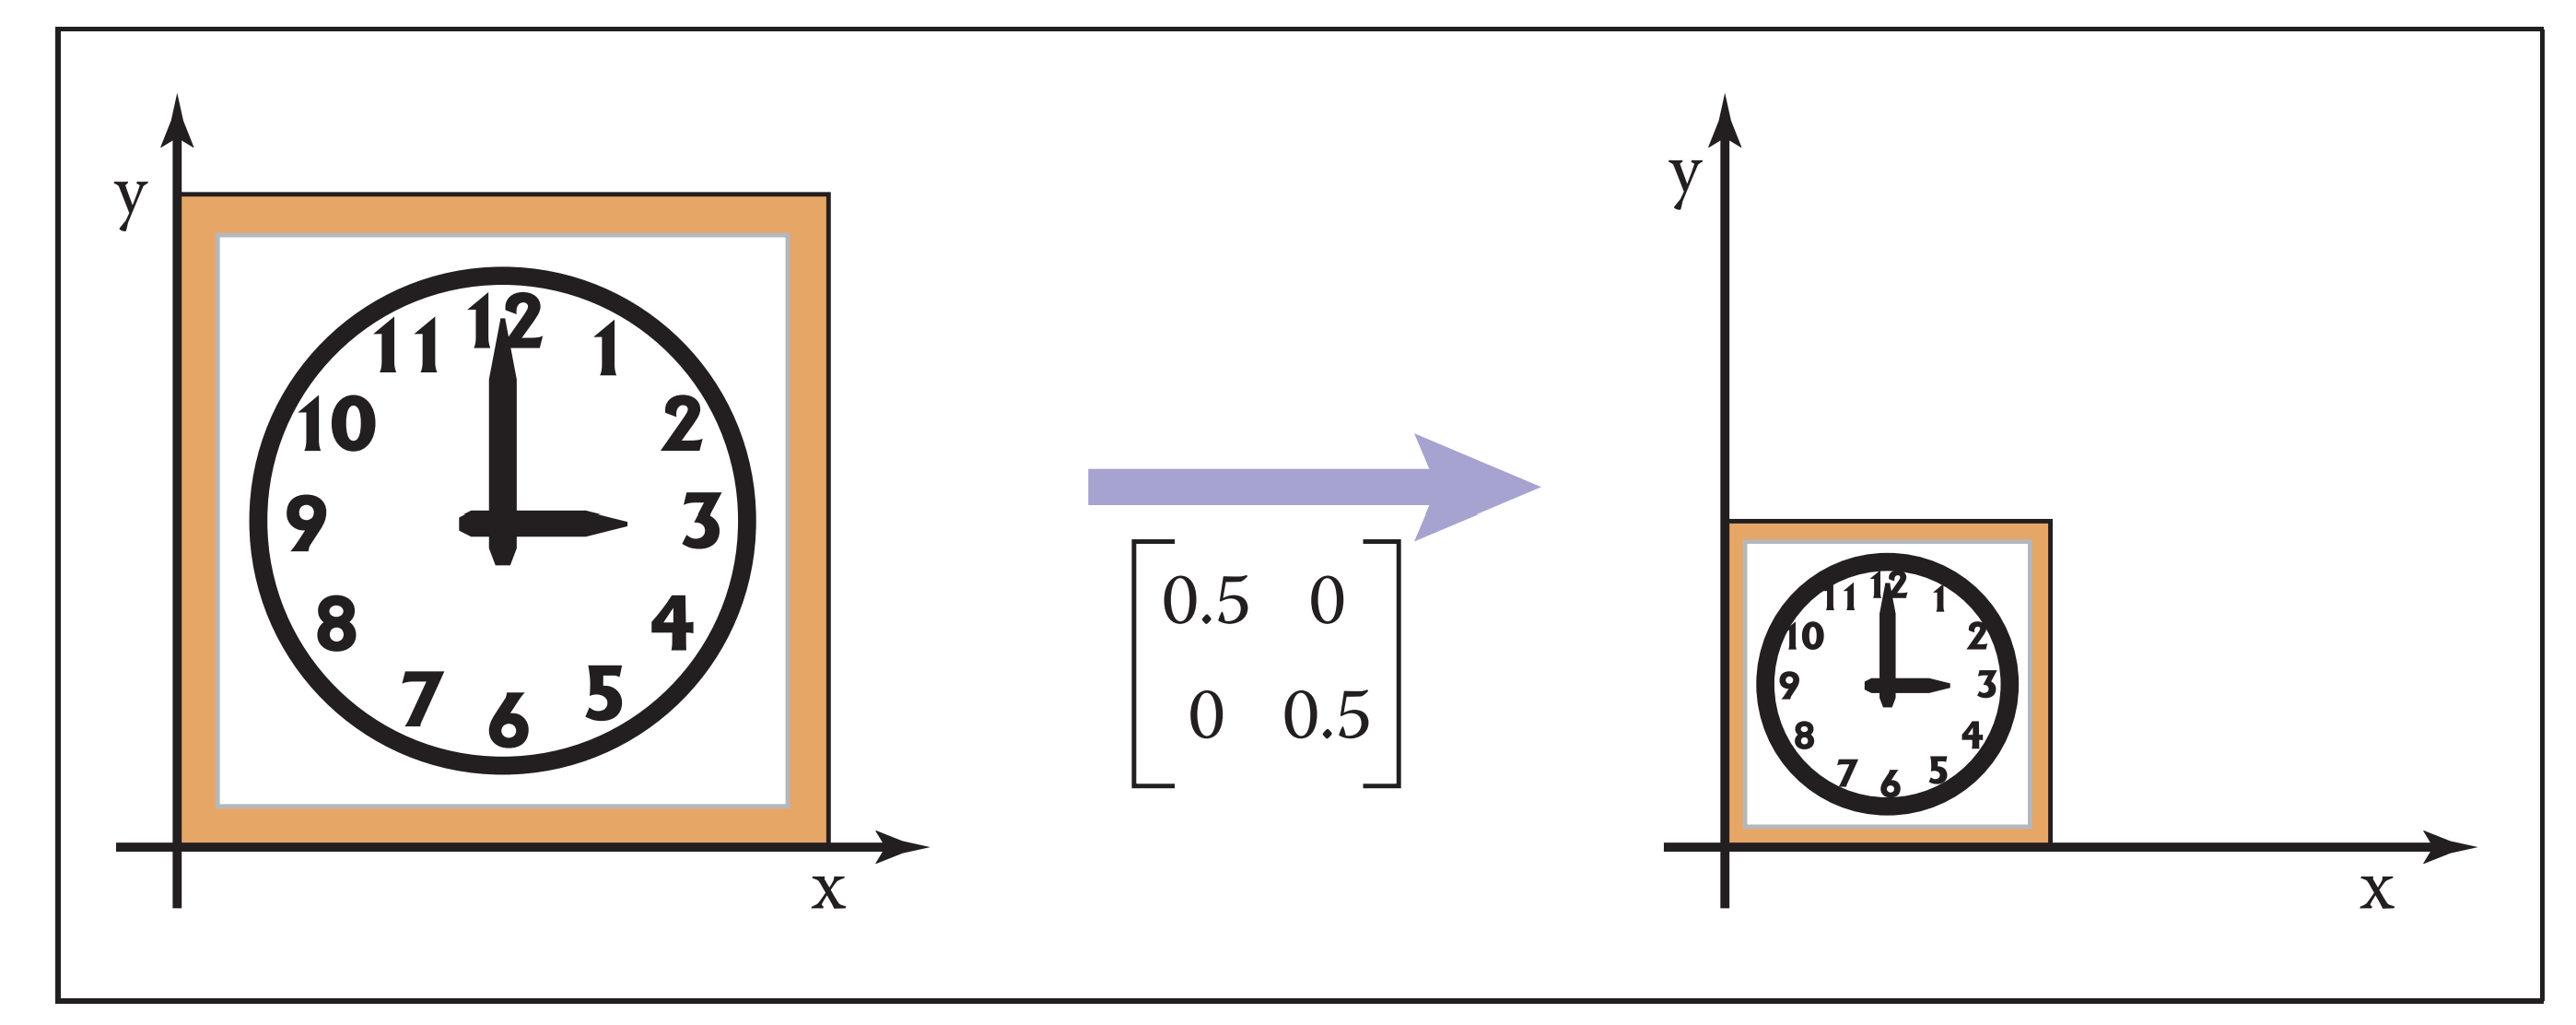
\includegraphics[scale=0.4]{Figure7.1.png}
	\caption{每个轴均匀缩放一半:轴对齐的缩放矩阵,对角线元素是缩放比例,非对角线的元素是零。}
	\label{fig:7.1}
\end{figure}

水平方向减半,垂直方向增加三倍的矩阵为(图\ref{fig:7.2}):

	\begin{equation}
		\operatorname{scale}\left(0.5, 1.5 \right)=\left[\begin{array}{cc}
			0.5 & 0 \\
			0 & 1.5
		\end{array}\right]
		\nonumber
	\end{equation}

\begin{figure}[htbp]
	\centering
	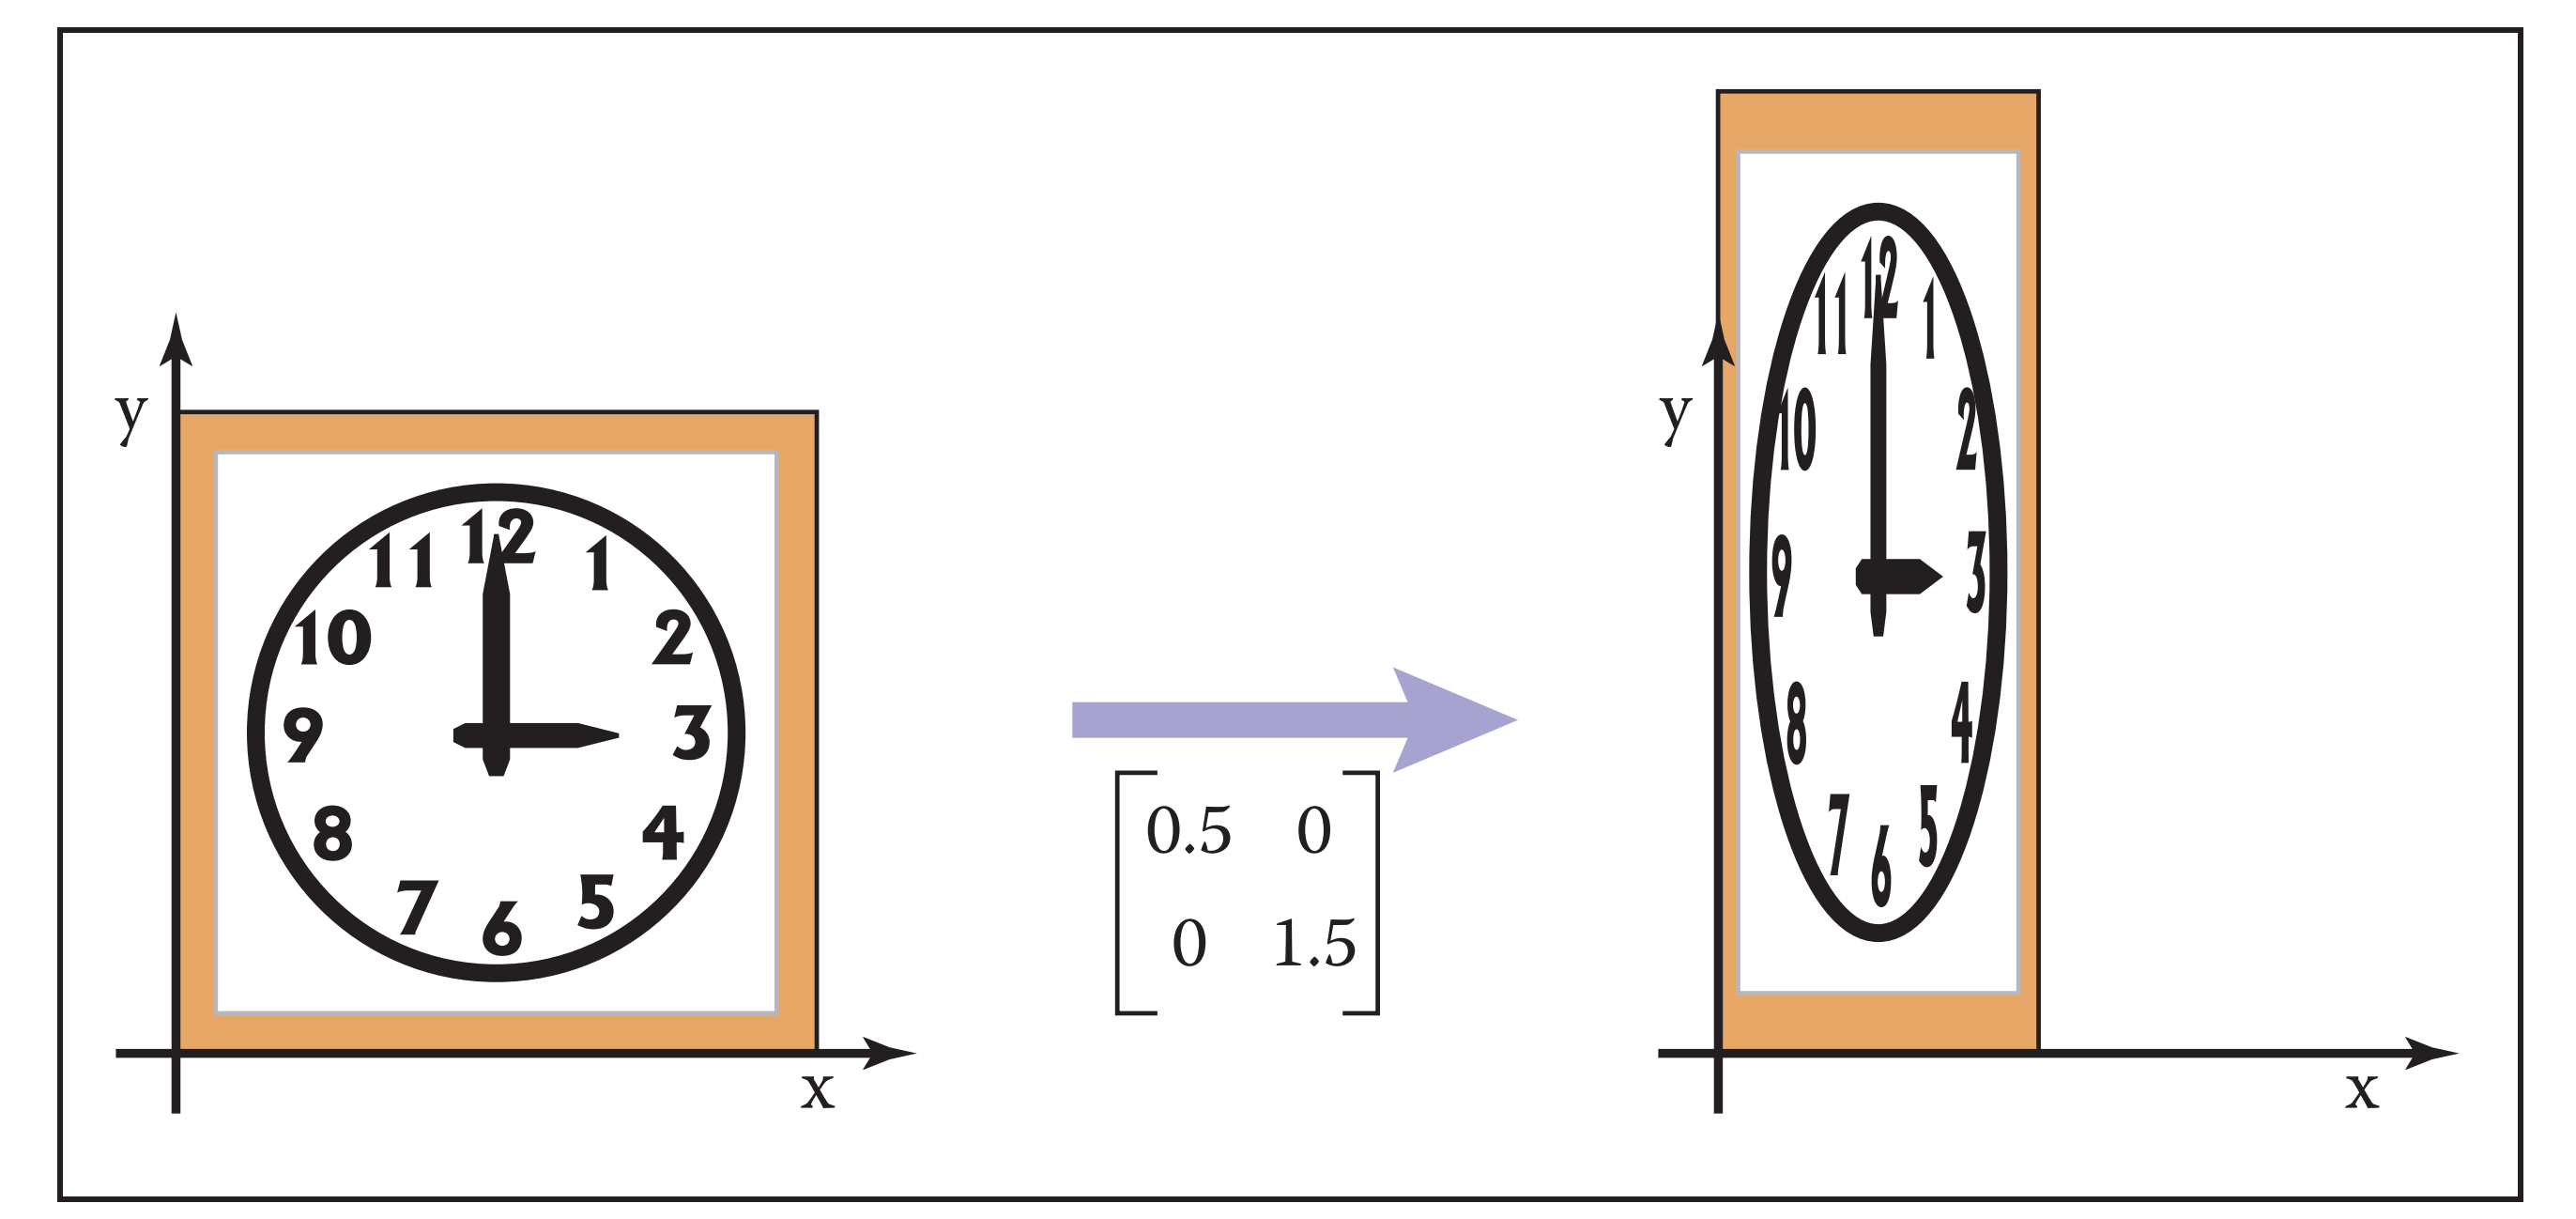
\includegraphics[scale=0.41]{Figure7.2.png}
	\caption{在x和y中不均匀缩放:缩放矩阵是对角阵,对角线元素不相等。注意到时钟的方形轮廓变为矩形,圆形则变为椭圆形。}
	\label{fig:7.2}
\end{figure}

\end{example}

\subsection{错切(Shearing)}

错切是一种将东西推向侧边,产生一种“摊牌”的效果。最下面的牌保持不动,牌越靠近牌顶,移动得越多。水平和垂直的错切矩阵是:

\begin{equation}
	\operatorname{shear-x}(s)=\left[\begin{array}{ll}
		1 & s \\
		0 & 1
	\end{array}\right], \quad \text { shear-y }(s)=\left[\begin{array}{ll}
		1 & 0 \\
		s & 1
	\end{array}\right]
\nonumber
\end{equation}

\begin{example}
	水平错切使垂直线变成向右倾斜45度线的变换是(如图\ref{fig:7.3}):
	\begin{equation}
		\operatorname{shear-x}(1)=\left[\begin{array}{ll}
			1 & 1 \\
			0 & 1
		\end{array}\right]
		\nonumber
	\end{equation}

\begin{figure}[htbp]
	\centering
	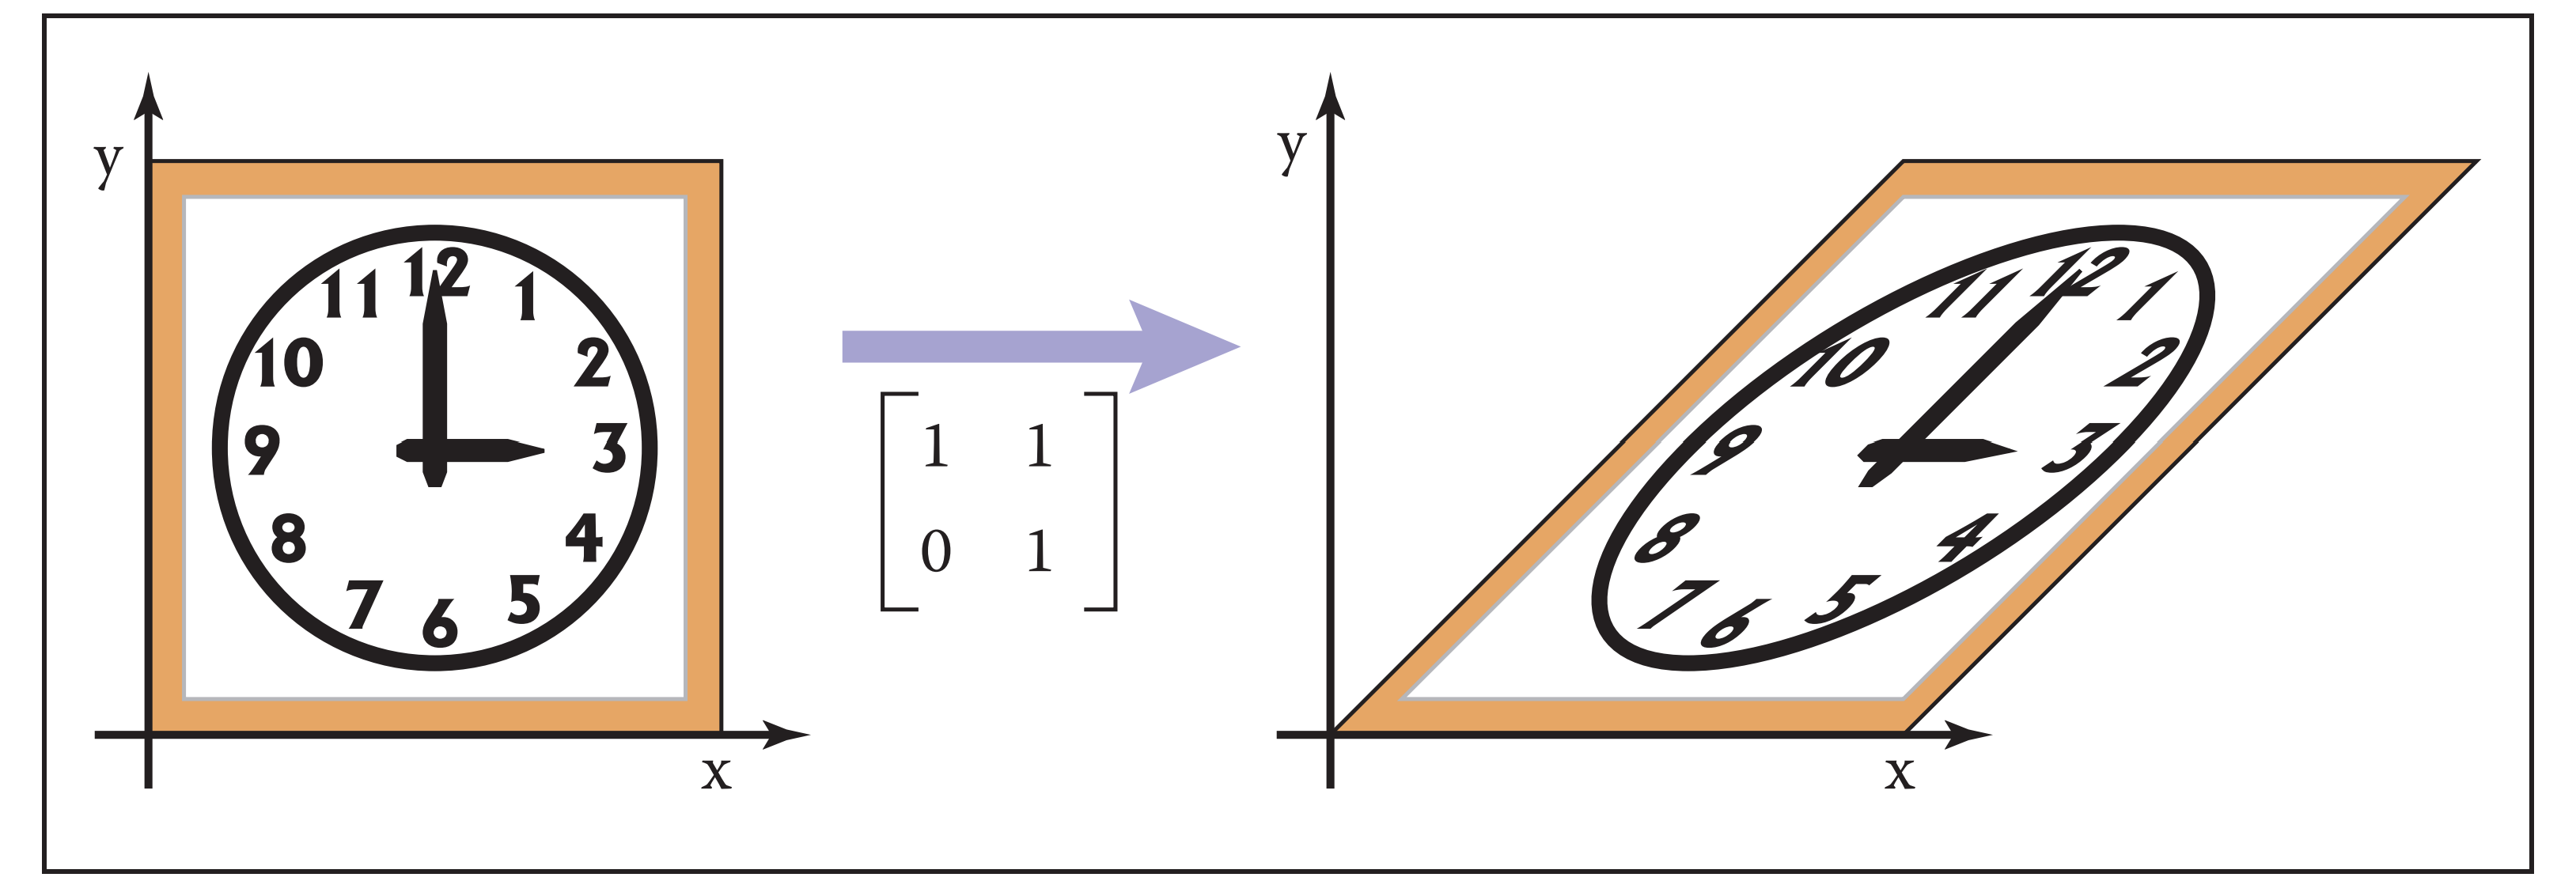
\includegraphics[scale=0.4]{Figure7.3.png}
	\caption{x错切矩阵将点向右移动,按点在y坐标位置的比例。如此,时钟的正方形轮廓变成了平行四边形,而随着缩放,时钟的圆形表面变成了椭圆。}
	\label{fig:7.3}
\end{figure}
	
\begin{figure}[htbp]
	\centering
	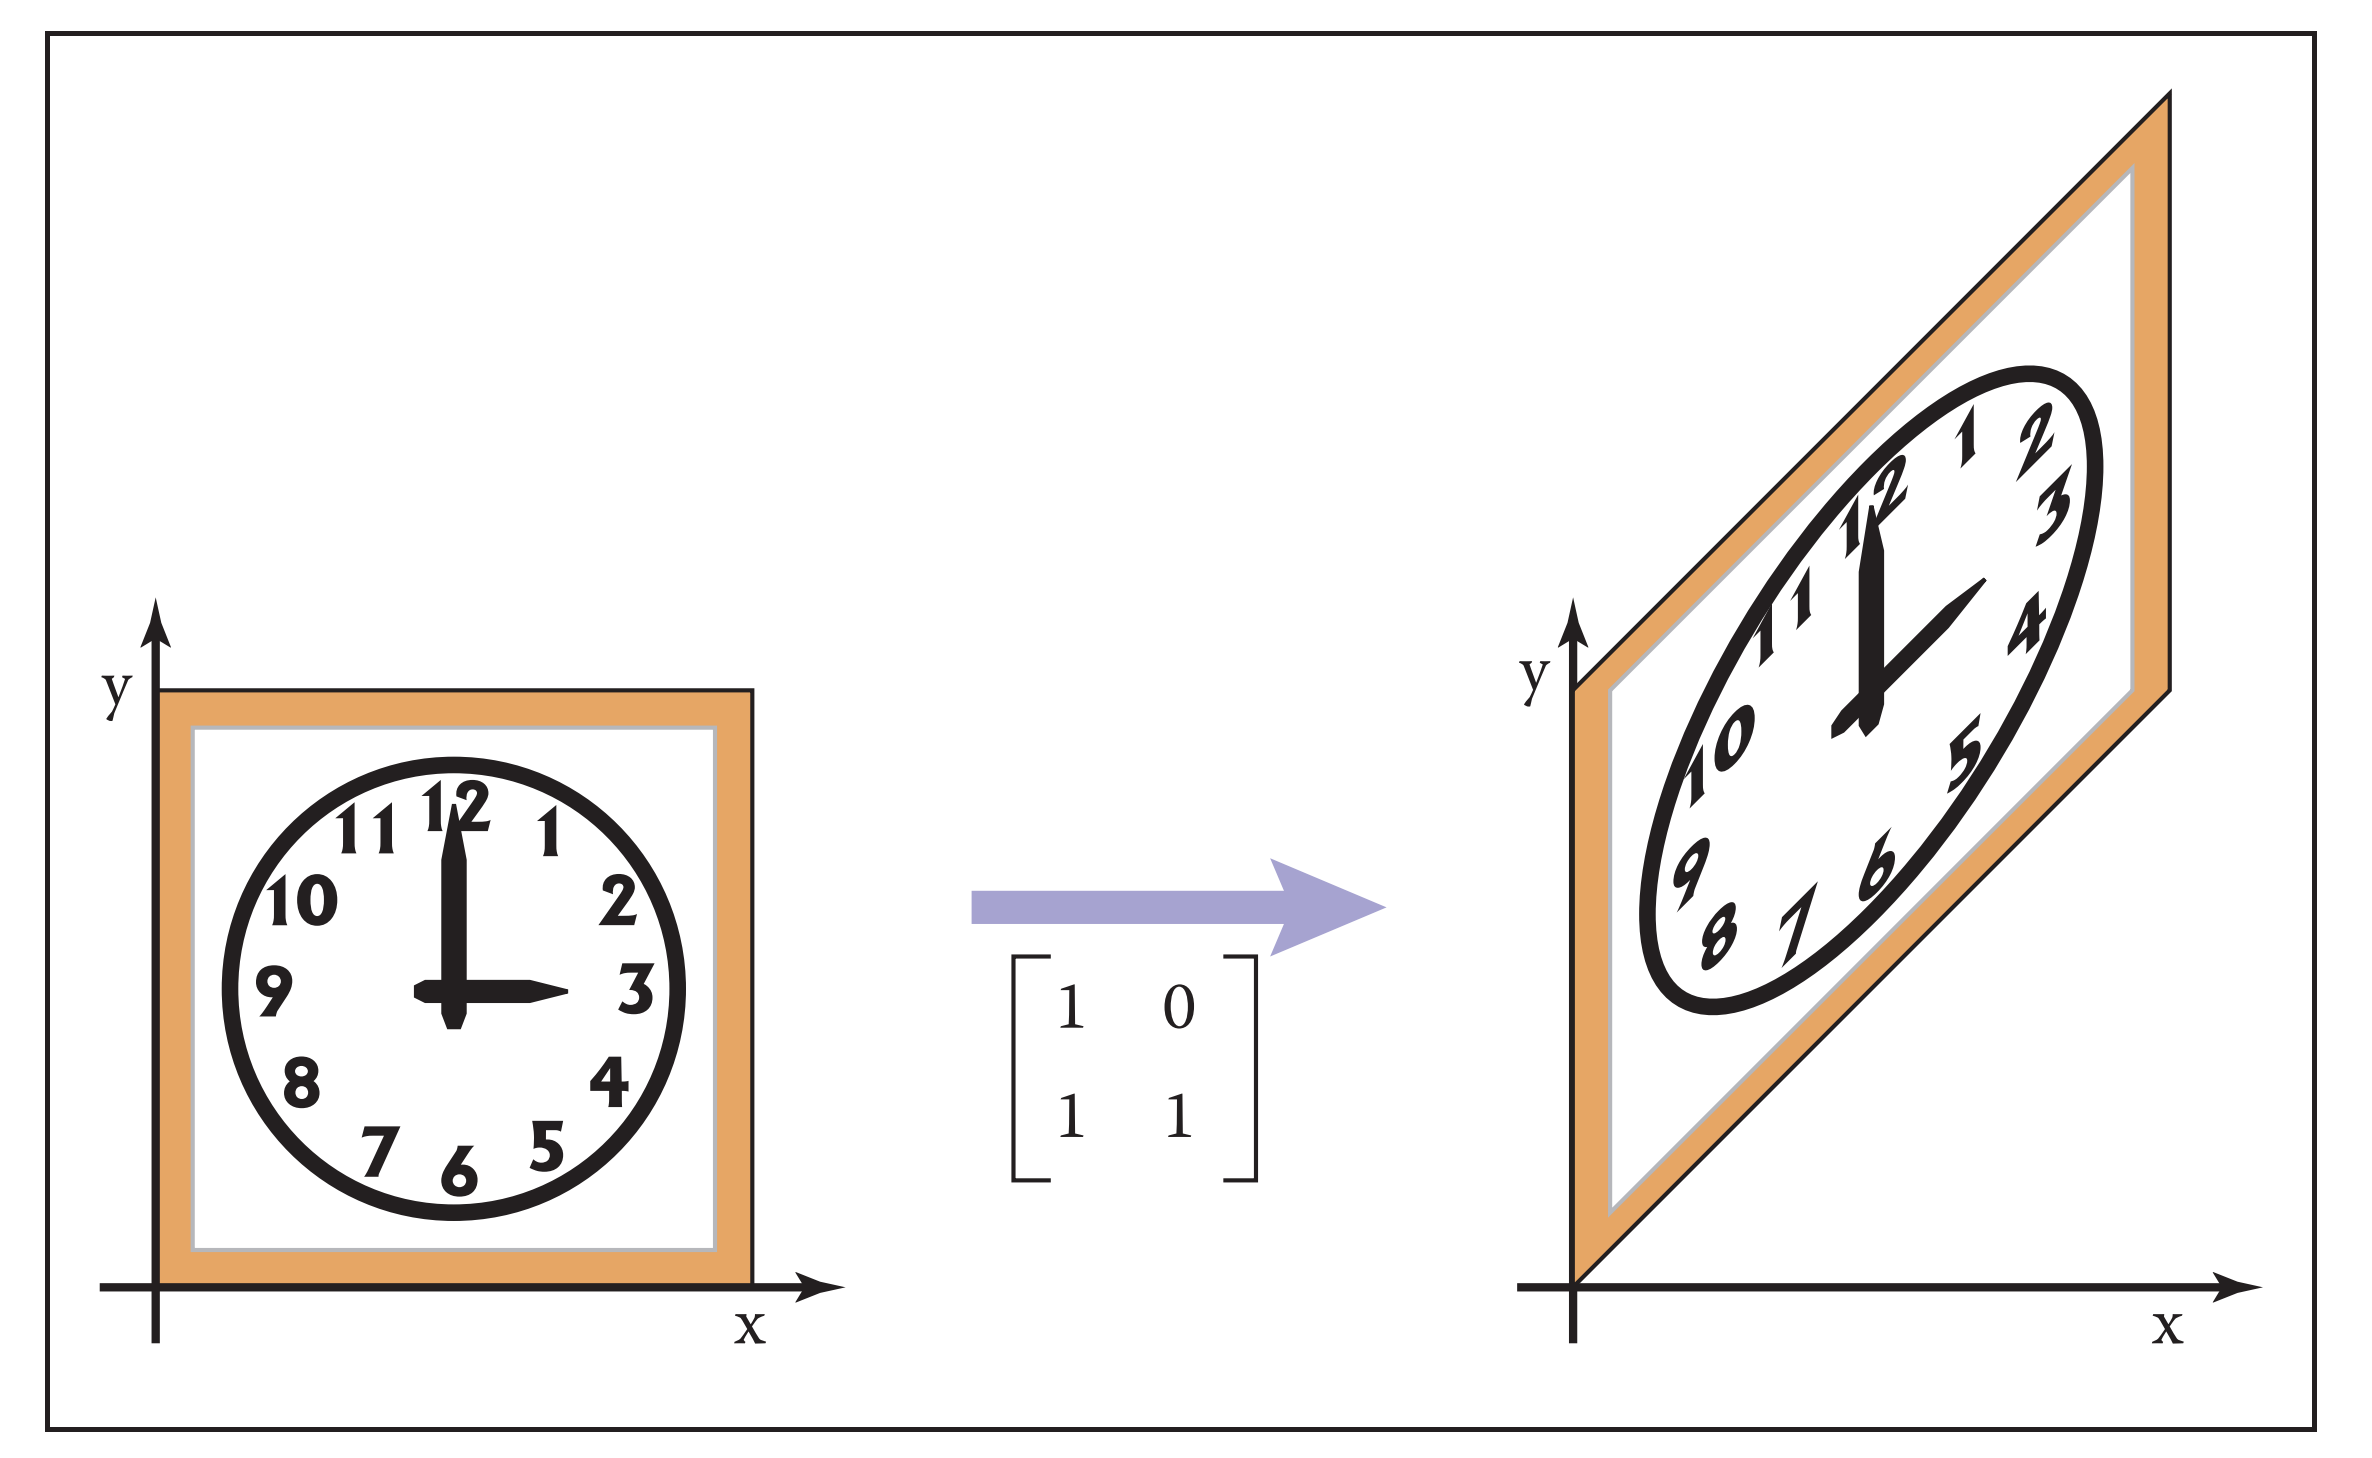
\includegraphics[scale=0.5]{Figure7.4.png}
	\caption{y错切矩阵将点向上移动,按照点在x坐标位置的比例。}
	\label{fig:7.4}
\end{figure}	
	
	垂直方向上类似的变换是(如图\ref{fig:7.4}):
	
	\begin{equation}
		\operatorname{shear-y}(1)=\left[\begin{array}{ll}
			1 & 0 \\
			1 & 1
		\end{array}\right]
		\nonumber
	\end{equation}
	
	在这两种情况下,时钟的正方形轮廓变成平行四边形,而时钟的圆形表盘外轮廓变成椭圆形\footnote{事实上,任何矩阵变换下的圆的图像都是椭圆。}。
	
	另一种考虑错切的方式是仅考虑垂直(或水平)轴的旋转。取垂直轴并顺时针倾斜角度$\phi$的错切变换为:
	
	\begin{equation}
		\left[\begin{array}{ll}
			1 &  \rm tan \phi \\
			0 & 1
		\end{array}\right]
		\nonumber
	\end{equation}

	类似地,将水平轴逆时针旋转角度$\phi$的错切矩阵为:
	
	\begin{equation}
		\left[\begin{array}{ll}
			1 &  0 \\
			\rm tan \phi & 1
		\end{array}\right]
		\nonumber
	\end{equation}
	
\end{example}

\subsection{旋转(Rotation)}

假设我们想逆时针旋转向量$\mathbf{a}$一个角度$\phi$,得到向量$\mathbf{b}$(如图\ref{fig:7.5})。如果$\mathbf{a}$与$x$轴成角度$\alpha$,其长度为$r=\sqrt{x_a^2+y_a^2}$,那么我们知道:

\begin{equation}
	\begin{aligned}
		& x_a=r \cos \alpha \\
		& y_a=r \sin \alpha
	\end{aligned}
\nonumber
\end{equation}

\begin{figure}[htbp]
	\centering
	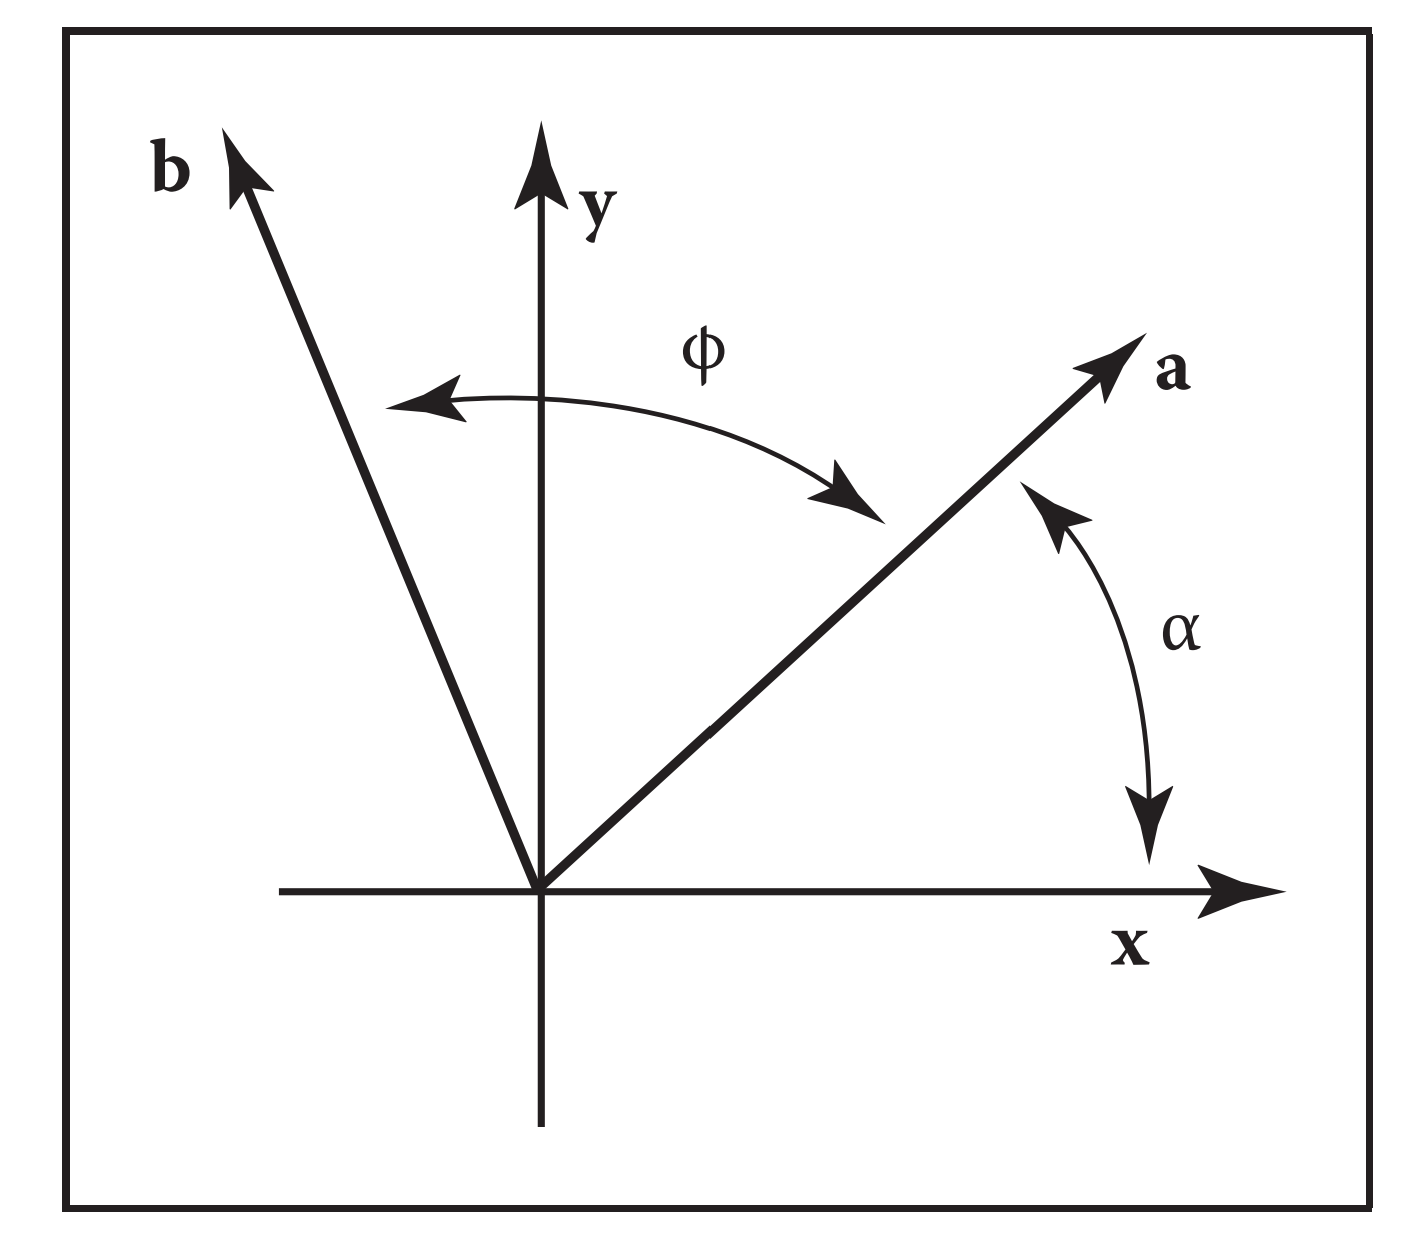
\includegraphics[scale=0.4]{Figure7.5.png}
	\caption{方程\ref{con:7.1}的几何图示}
	\label{fig:7.5}
\end{figure}	

因为$\mathbf{b}$是$\mathbf{a}$旋转而来,所以$\mathbf{b}$的长度也是$r$。$\mathbf{b}$是$\mathbf{a}$旋转$\phi$角度,所以$\mathbf{b}$与$x$轴之间的夹角是$(\alpha + \phi)$。使用三角加法恒等式(第\ref{label}小节):

\begin{equation}\label{con:7.1}
	\begin{aligned}
		& x_b=r \cos (\alpha+\phi)= r \cos \alpha \cos \phi-r \sin \alpha \sin \phi \\
		& y_b=r \sin (\alpha+\phi)= r \sin \alpha \cos \phi+r \cos \alpha \sin \phi
	\end{aligned}
\end{equation}

将$\mathbf{a}$向量带入式\ref{con:7.1},$x_a=r \cos \alpha$,$y_a=r \sin \alpha$,故可以得到:

\begin{equation}
	\begin{aligned}
		 x_b &= x_a \cos \phi - y_a \sin \phi \\
		 y_b &= y_a \cos \phi + x_a \sin \phi
	\end{aligned}
\nonumber
\end{equation}

所以从$\mathbf{a}$变换到$\mathbf{b}$的矩阵形式为:

\begin{equation}
	\operatorname{rotate}(\phi)=\left[\begin{array}{rr}
		\cos \phi & -\sin \phi \\
		\sin \phi & \cos \phi
	\end{array}\right]
\nonumber
\end{equation}

\begin{example}
	旋转$pi / 4$弧度($45^{\circ}$)的旋转矩阵是(如图\ref{fig:7.6}):
	\begin{equation}
		\left[\begin{array}{cr}
			\cos \frac{\pi}{4} & -\sin \frac{\pi}{4} \\
			\sin \frac{\pi}{4} & \cos \frac{\pi}{4}
		\end{array}\right]=\left[\begin{array}{rr}
			0.707 & -0.707 \\
			0.707 & 0.707
		\end{array}\right] \text {. }
	\end{equation}
	
	\begin{figure}[htbp]
		\centering
		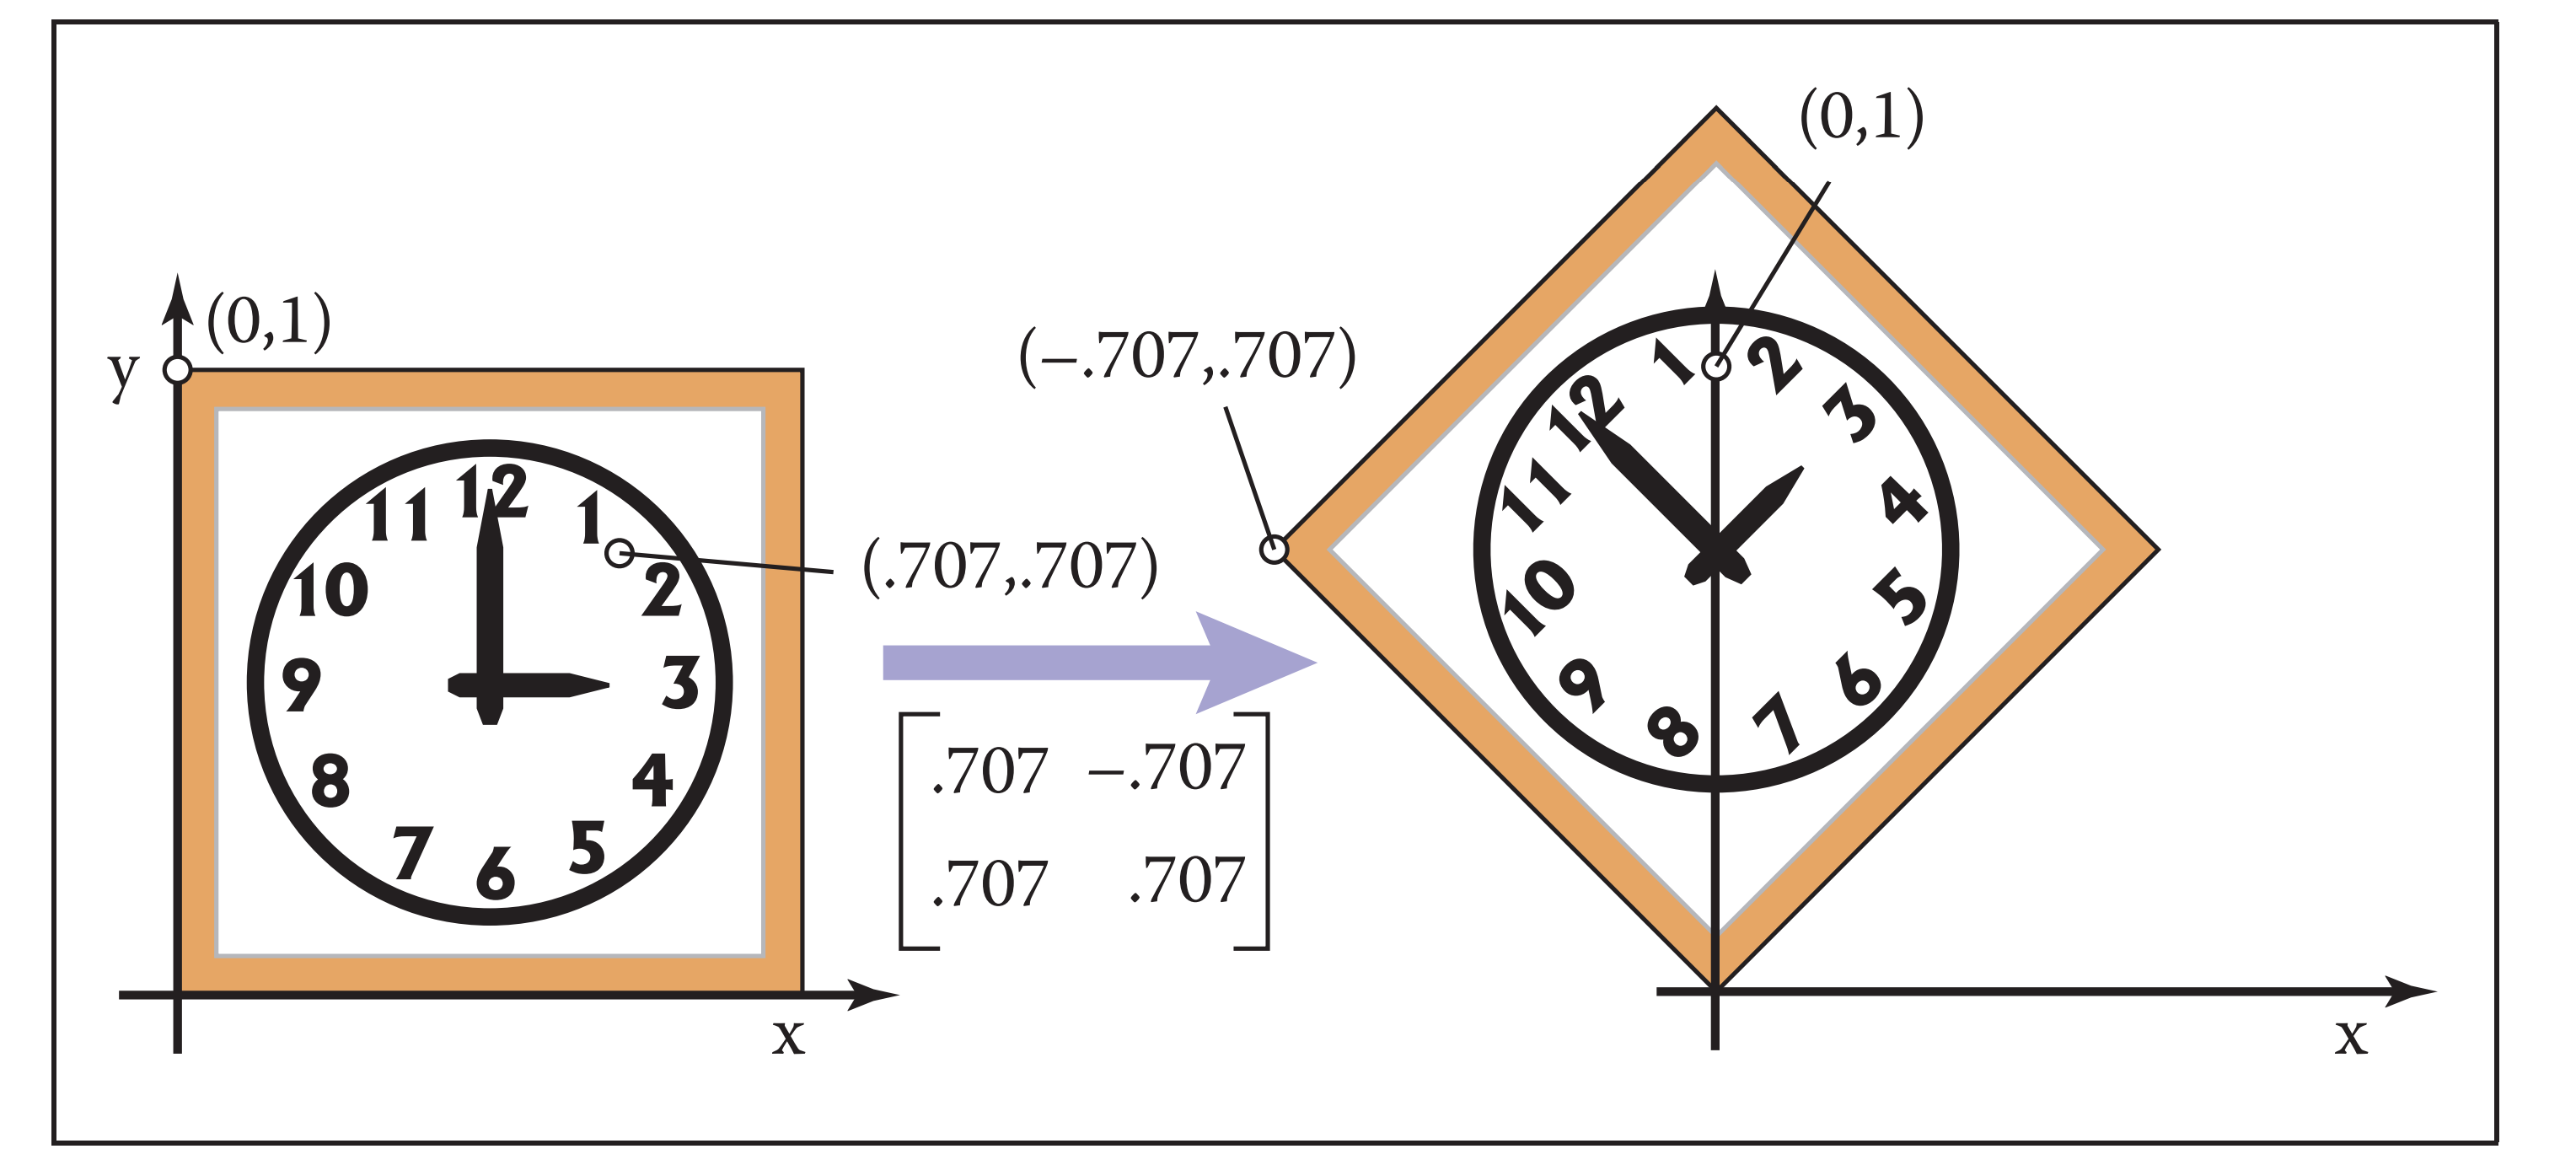
\includegraphics[scale=0.4]{Figure7.6.png}
		\caption{旋转$45^{\circ}$。注意到旋转是逆时针的,$cos(45^{\circ}) = sin(45^{\circ}) \approx .707 $}
		\label{fig:7.6}
	\end{figure}	
	
	顺时针方向旋转$\pi / 6$弧度($30^{\circ}$),在我们的框架中是旋转$-\pi / 6$弧度的旋转矩阵(如图\ref{fig:7.7}):
	
	\begin{equation}
		\left[\begin{array}{cr}
			\cos \frac{-\pi}{6} & -\sin \frac{-\pi}{6} \\
			\sin \frac{-\pi}{6} & \cos \frac{-\pi}{6}
		\end{array}\right]=\left[\begin{array}{rr}
			0.866 & 0.5 \\
			-0.5 & 0.866
		\end{array}\right] \text {. }
	\end{equation}
	
	\begin{figure}[htbp]
		\centering
		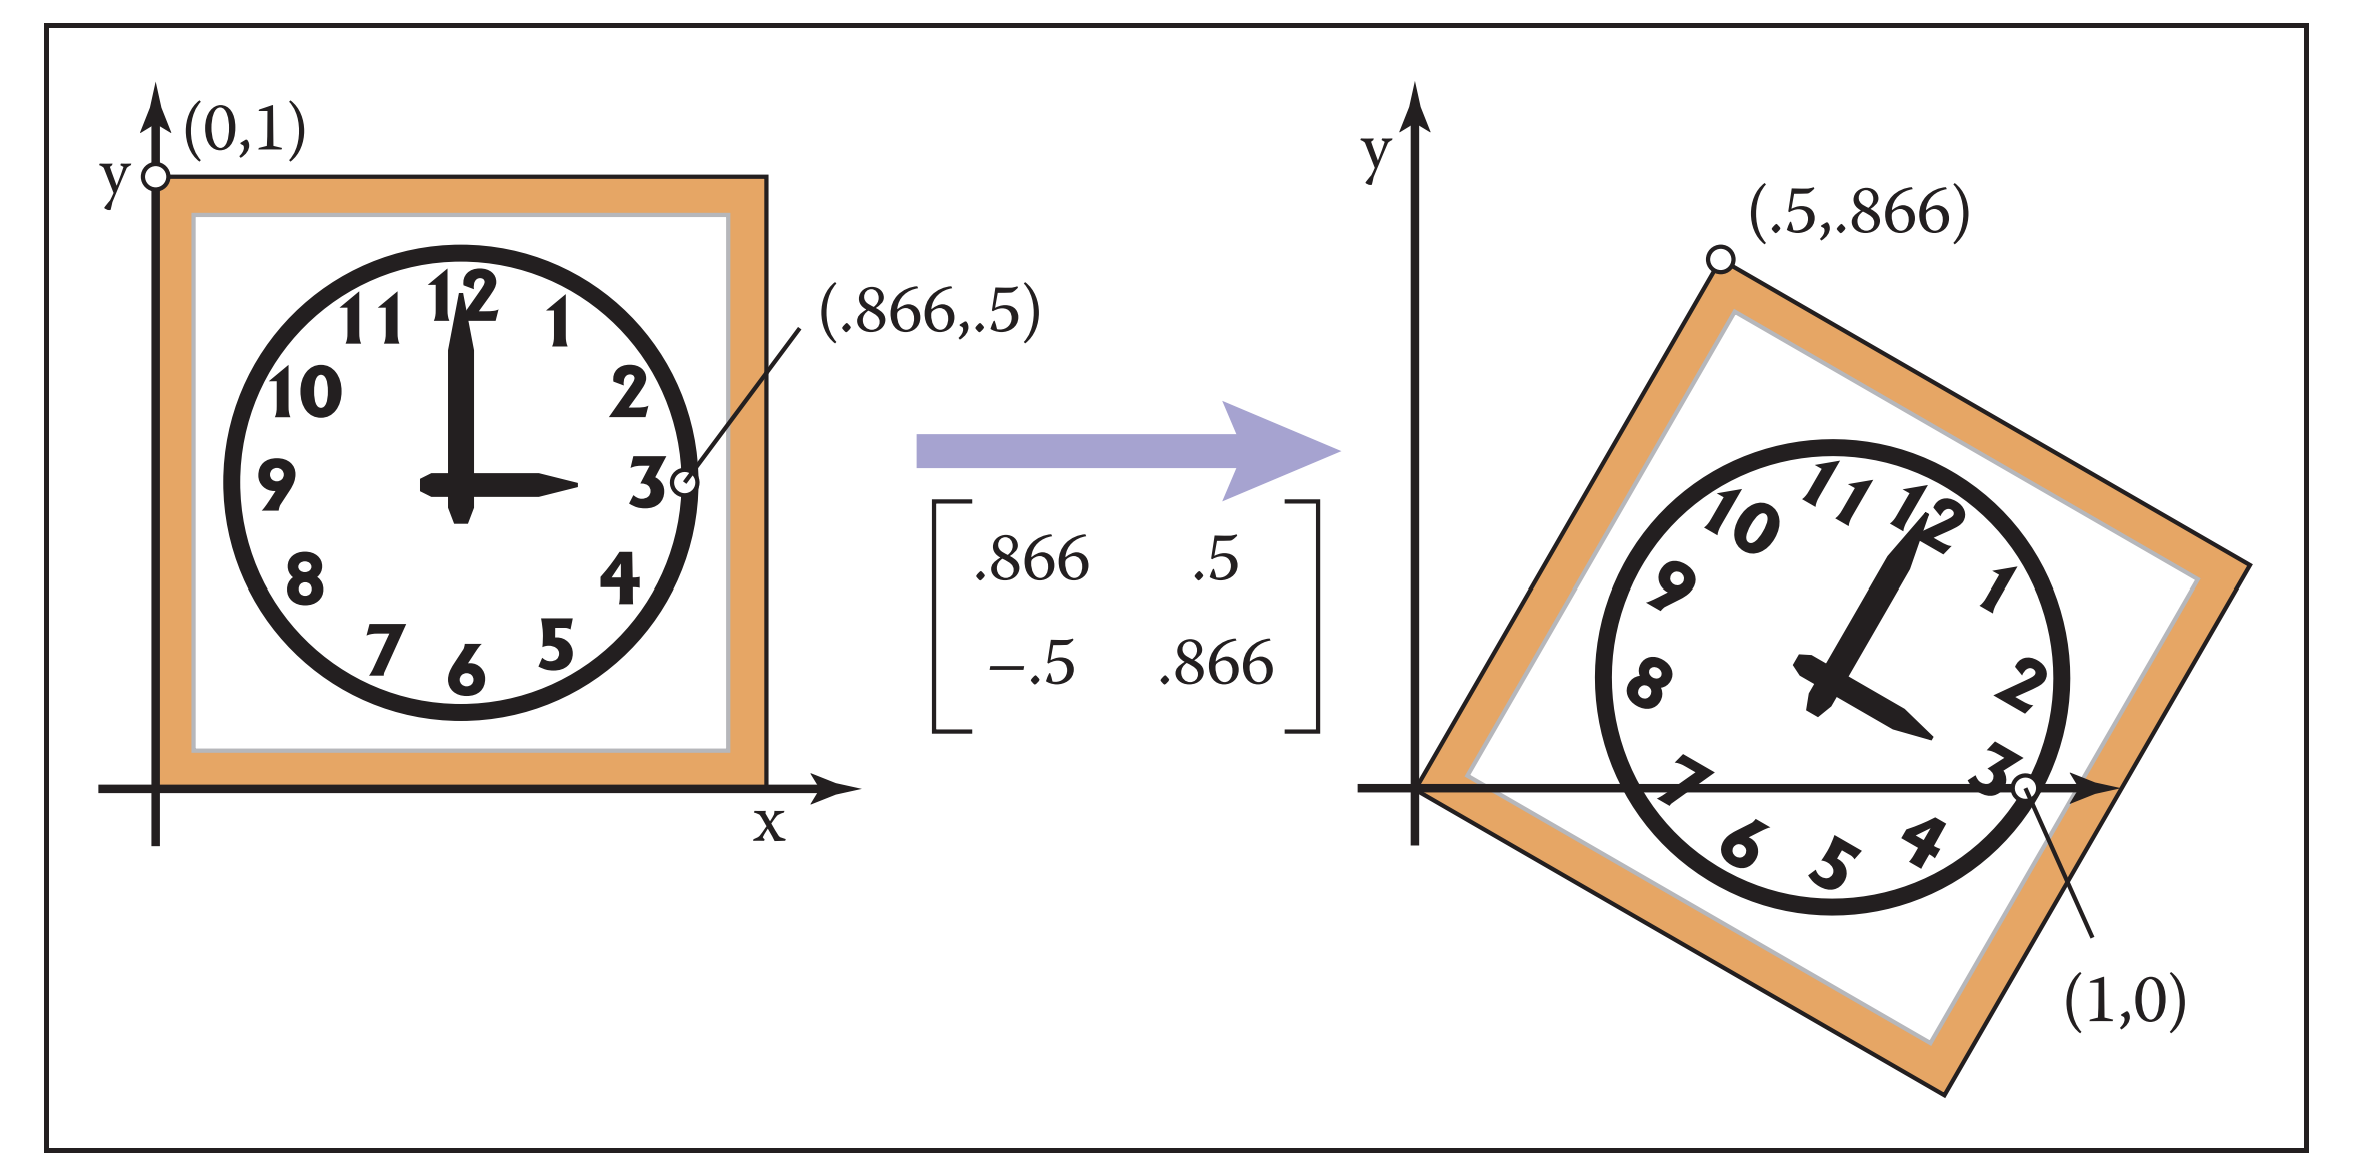
\includegraphics[scale=0.5]{Figure7.7.png}
		\caption{旋转$-30^{\circ}$。注意到旋转方向为顺时针,$cos(-30^{\circ}) \approx .866 $和$sin(-30^{\circ}) \approx -.5 $。}
		\label{fig:7.7}
	\end{figure}	
	
	
\end{example}

因为旋转矩阵每一行的范数是1$\left(\sin ^2 \phi+\cos ^2 \phi=1\right)$,并且行是正交的$(\cos \phi(-\sin \phi)+\sin \phi \cos \phi=0)$,我们看到旋转矩阵是正交矩阵(第\ref{5.2.4}节)。观察矩阵我们可以读出两对正交向量:两个列向量,(没看懂。。。)

\subsection{反射(Reflection)}

我们可以通过使用有一个负比例因子的比例矩阵来反射任一坐标轴上的向量(如图\ref{fig:7.8},图\ref{fig:7.9}):

\begin{equation}
	\text { reflect-y }=\left[\begin{array}{rr}
		-1 & 0 \\
		0 & 1
	\end{array}\right], \quad \text { reflect-x }=\left[\begin{array}{rr}
		1 & 0 \\
		0 & -1
	\end{array}\right]
\nonumber
\end{equation}

\begin{figure}[htbp]
	\centering
	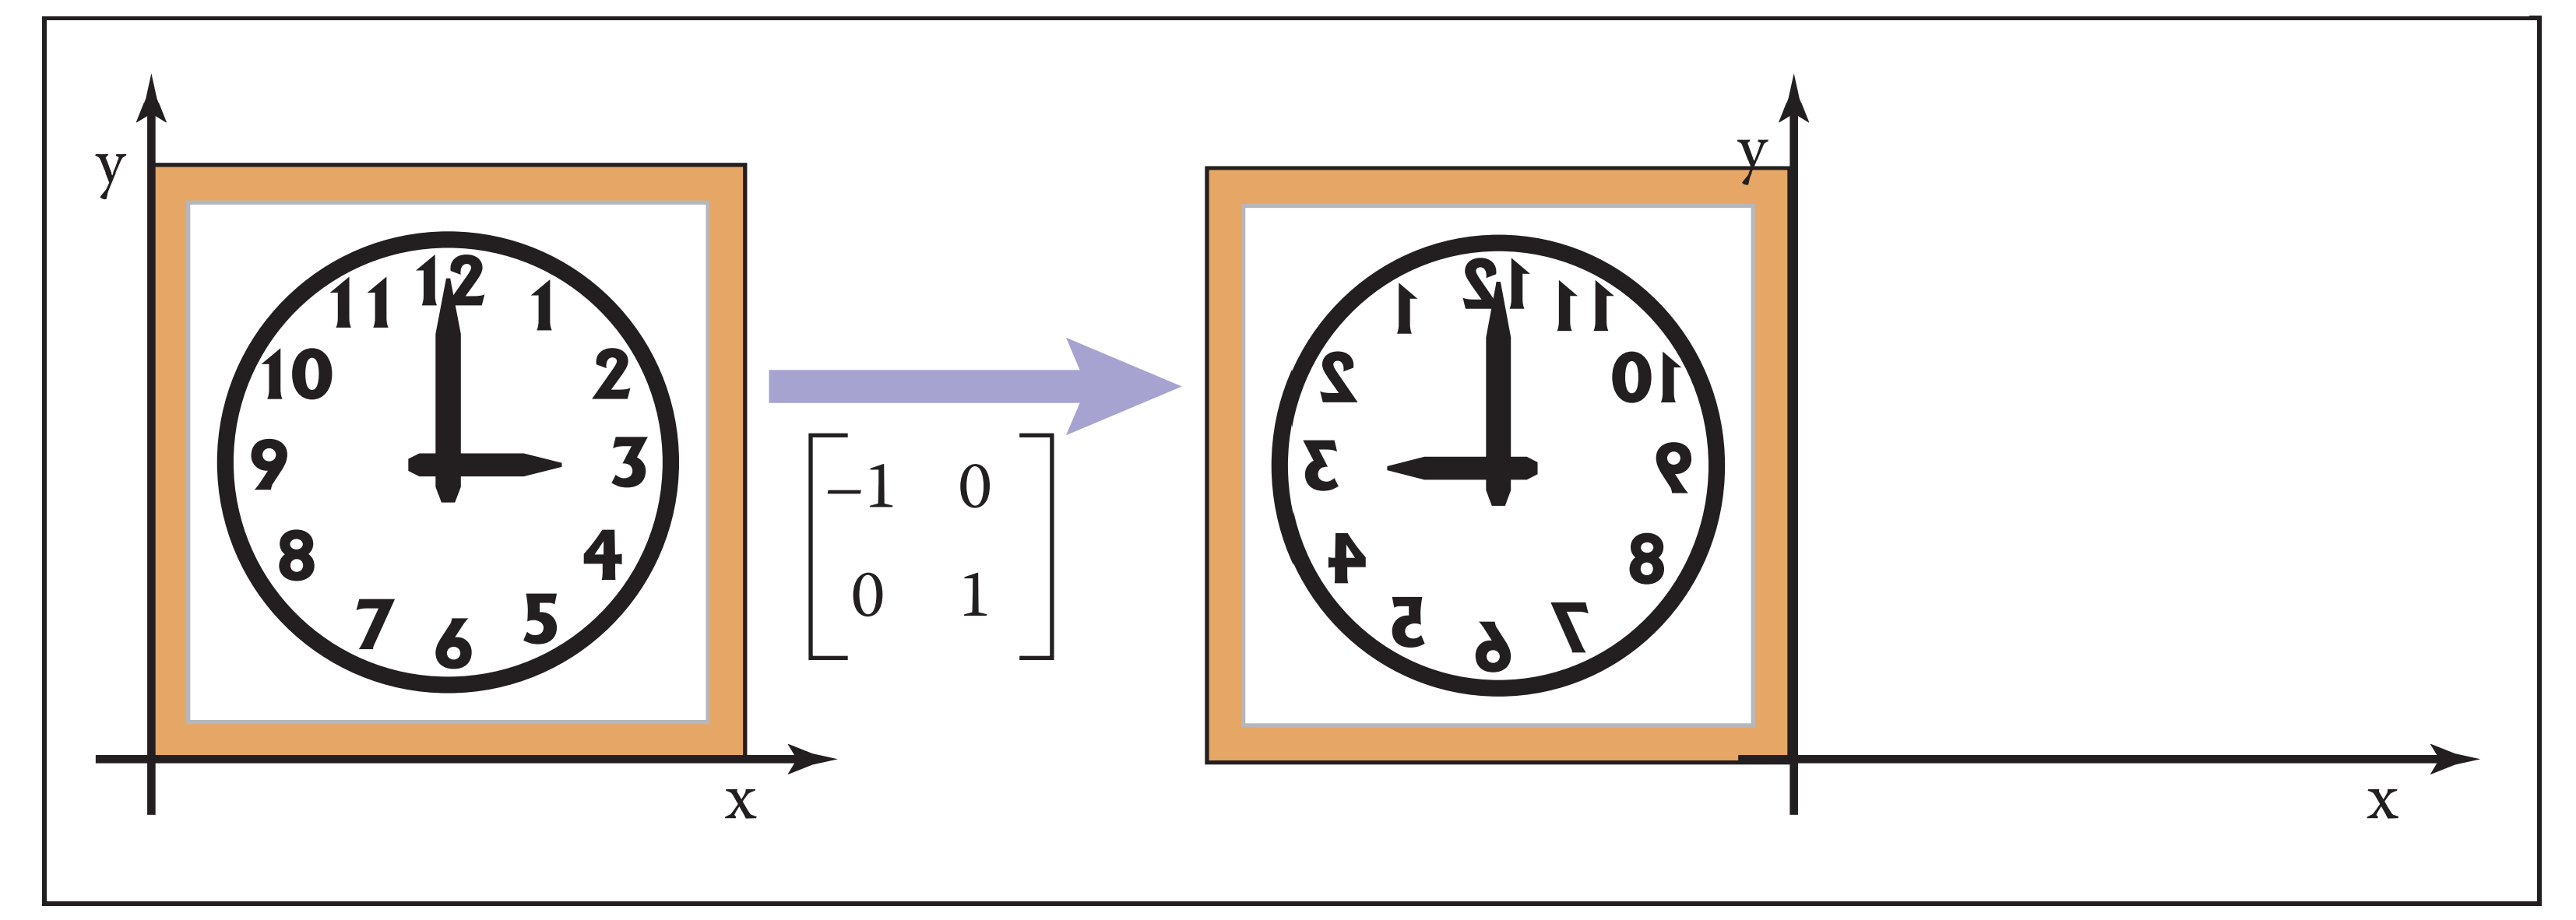
\includegraphics[scale=0.4]{Figure7.8.png}
	\caption{通过将所有x坐标乘以–1来实现关于y轴的反射。}
	\label{fig:7.8}
\end{figure}	

\begin{figure}[htbp]
	\centering
	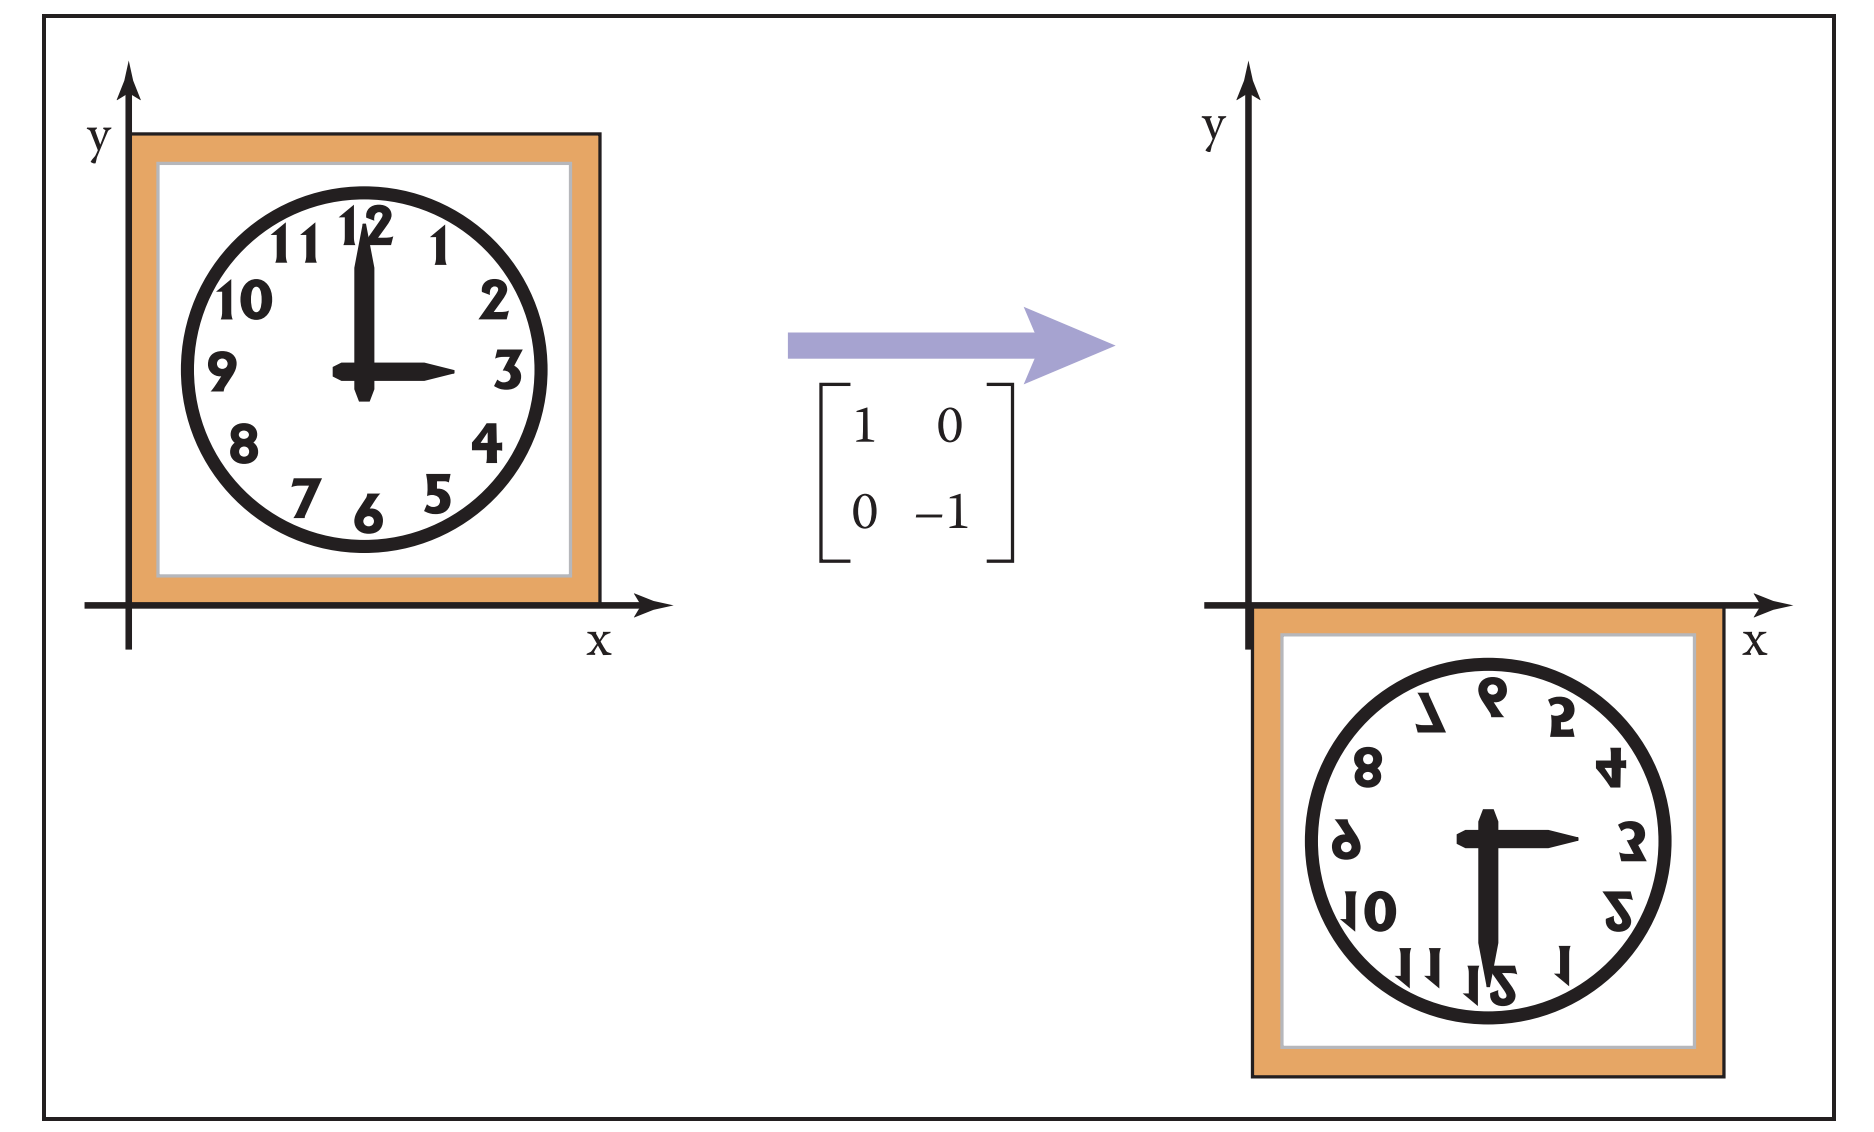
\includegraphics[scale=0.4]{Figure7.9.png}
	\caption{通过将所有y坐标乘以–1来实现关于x轴的反射。}
	\label{fig:7.9}
\end{figure}	

虽然人们可能会认为对角线的两个元素中都是−1的矩阵也是反射,但实际上它只是$\pi$弧度的旋转。

\subsection{变换的组成和分解(Composition and Decomposition of Transformations)}

图形程序通常对一个物体应用多个变换。例如,我们可能想先使用$\mathbf{S}$进行缩放,然后使用$\mathbf{R}$进行旋转。这将在二维向量$\mathbf{v}_{1}$上分两步完成:

\begin{equation}
	\text { first, } \mathbf{v}_2=\mathbf{S} \mathbf{v}_1, \text { then, } \mathbf{v}_3=\mathbf{R v}_2
	\nonumber
\end{equation}

另一种书写方式为:

\begin{equation}
	\mathbf{v}_3=\mathbf{R}\left(\mathbf{S v}_1\right)
	\nonumber
\end{equation}

因为矩阵乘法是满足结合律的,所以我们也可以写为:

\begin{equation}
	\mathbf{v}_3=(\mathbf{R S}) \mathbf{v}_1
	\nonumber
\end{equation}

换言之,我们可以使用相同大小的单个矩阵来表示由两个矩阵对向量变换的效果,我们可以将两个矩阵相乘来得到这个矩阵:$\mathbf{M}=\mathbf{R S}$(如图\ref{fig:7.10})。

请记住这些变换是从右侧进行变换的,这非常重要。所以矩阵$\mathbf{M}=\mathbf{R S}$先应用$\mathbf{S}$后应用$\mathbf{R}$。

\begin{figure}[htbp]
	\centering
	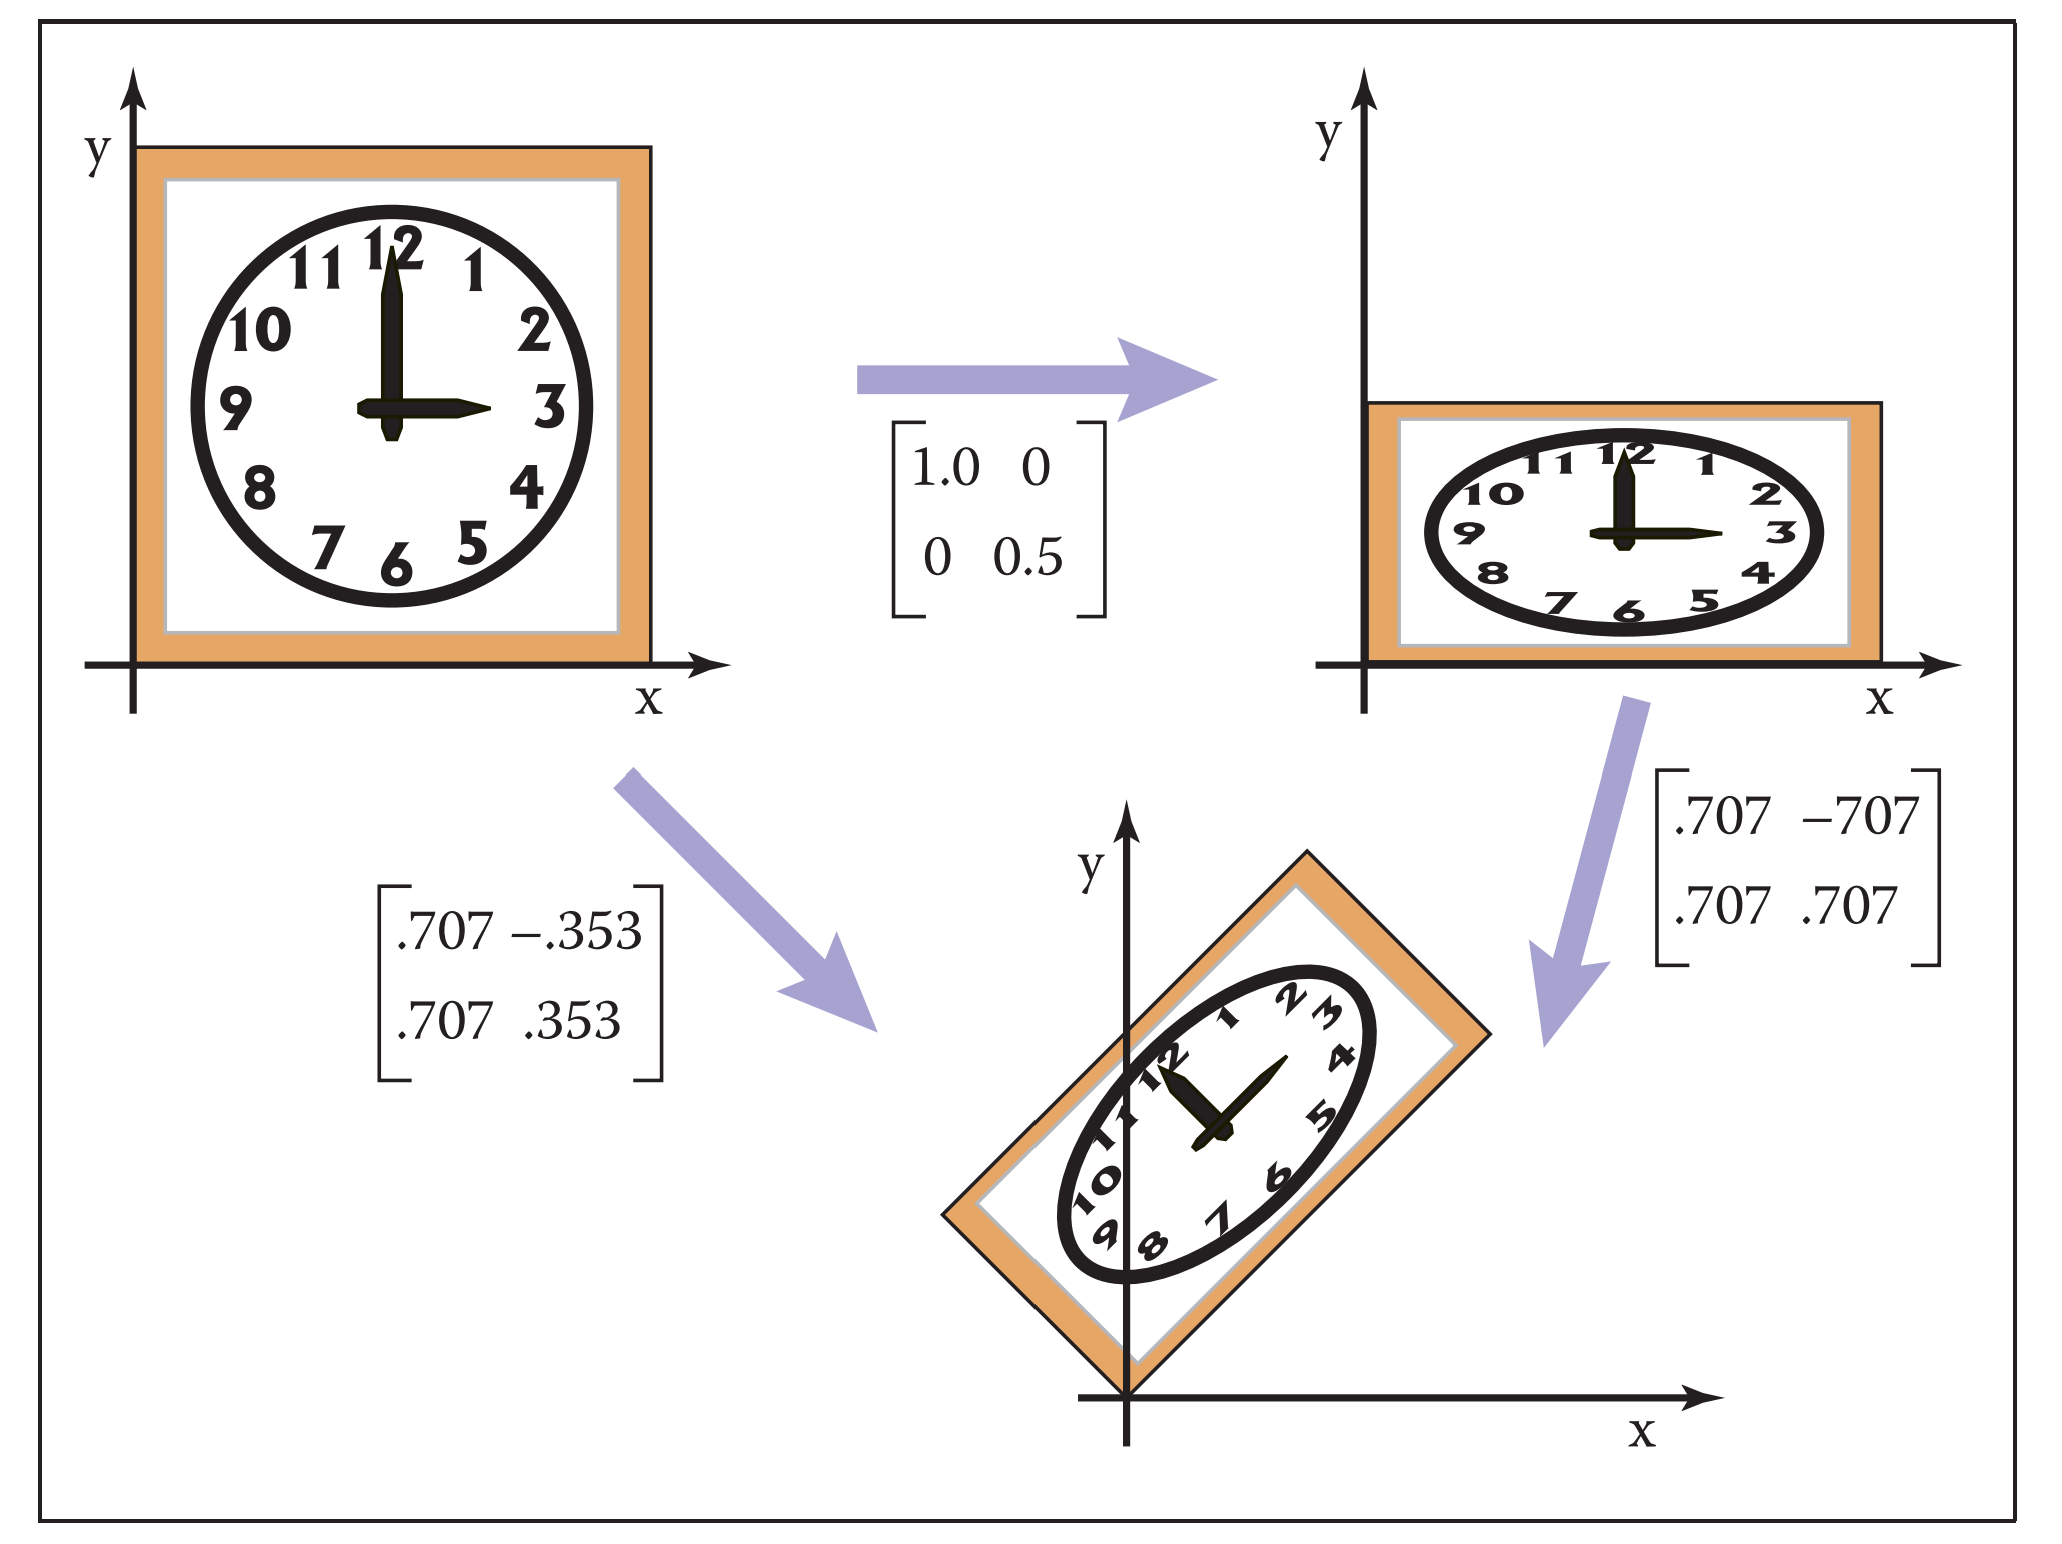
\includegraphics[scale=0.4]{Figure7.10.png}
	\caption{依次应用两个变换矩阵与应用一次这些矩阵的乘积是一样的。这是一个十分关键的概念,是大多数图形硬件和软件的基础。}
	\label{fig:7.10}
\end{figure}	

\begin{example}
	假设我们想在垂直方向上缩放一半,然后旋转$\pi/4$弧度($45^{\circ}$),其变换矩阵为:
	
	\begin{equation}
		\left[\begin{array}{cr}
			0.707 & -0.707 \\
			0.707 & 0.707
		\end{array}\right]\left[\begin{array}{cc}
			1 & 0 \\
			0 & 0.5
		\end{array}\right]=\left[\begin{array}{cc}
			0.707 & -0.353 \\
			0.707 & 0.353
		\end{array}\right]
	\nonumber
	\end{equation}

请务必记住矩阵乘法不是可交换的。所以变换的顺序很重要。对于这个例子,先进行旋转再进行缩放,是不同的变换矩阵(如图\ref{fig:7.11}):

\begin{equation}
	\left[\begin{array}{cc}
		1 & 0 \\
		0 & 0.5
	\end{array}\right]\left[\begin{array}{cr}
		0.707 & -0.707 \\
		0.707 & 0.707
	\end{array}\right]=\left[\begin{array}{rr}
		0.707 & -0.707 \\
		0.353 & 0.353
	\end{array}\right]
\nonumber
\end{equation}

\begin{figure}[htbp]
	\centering
	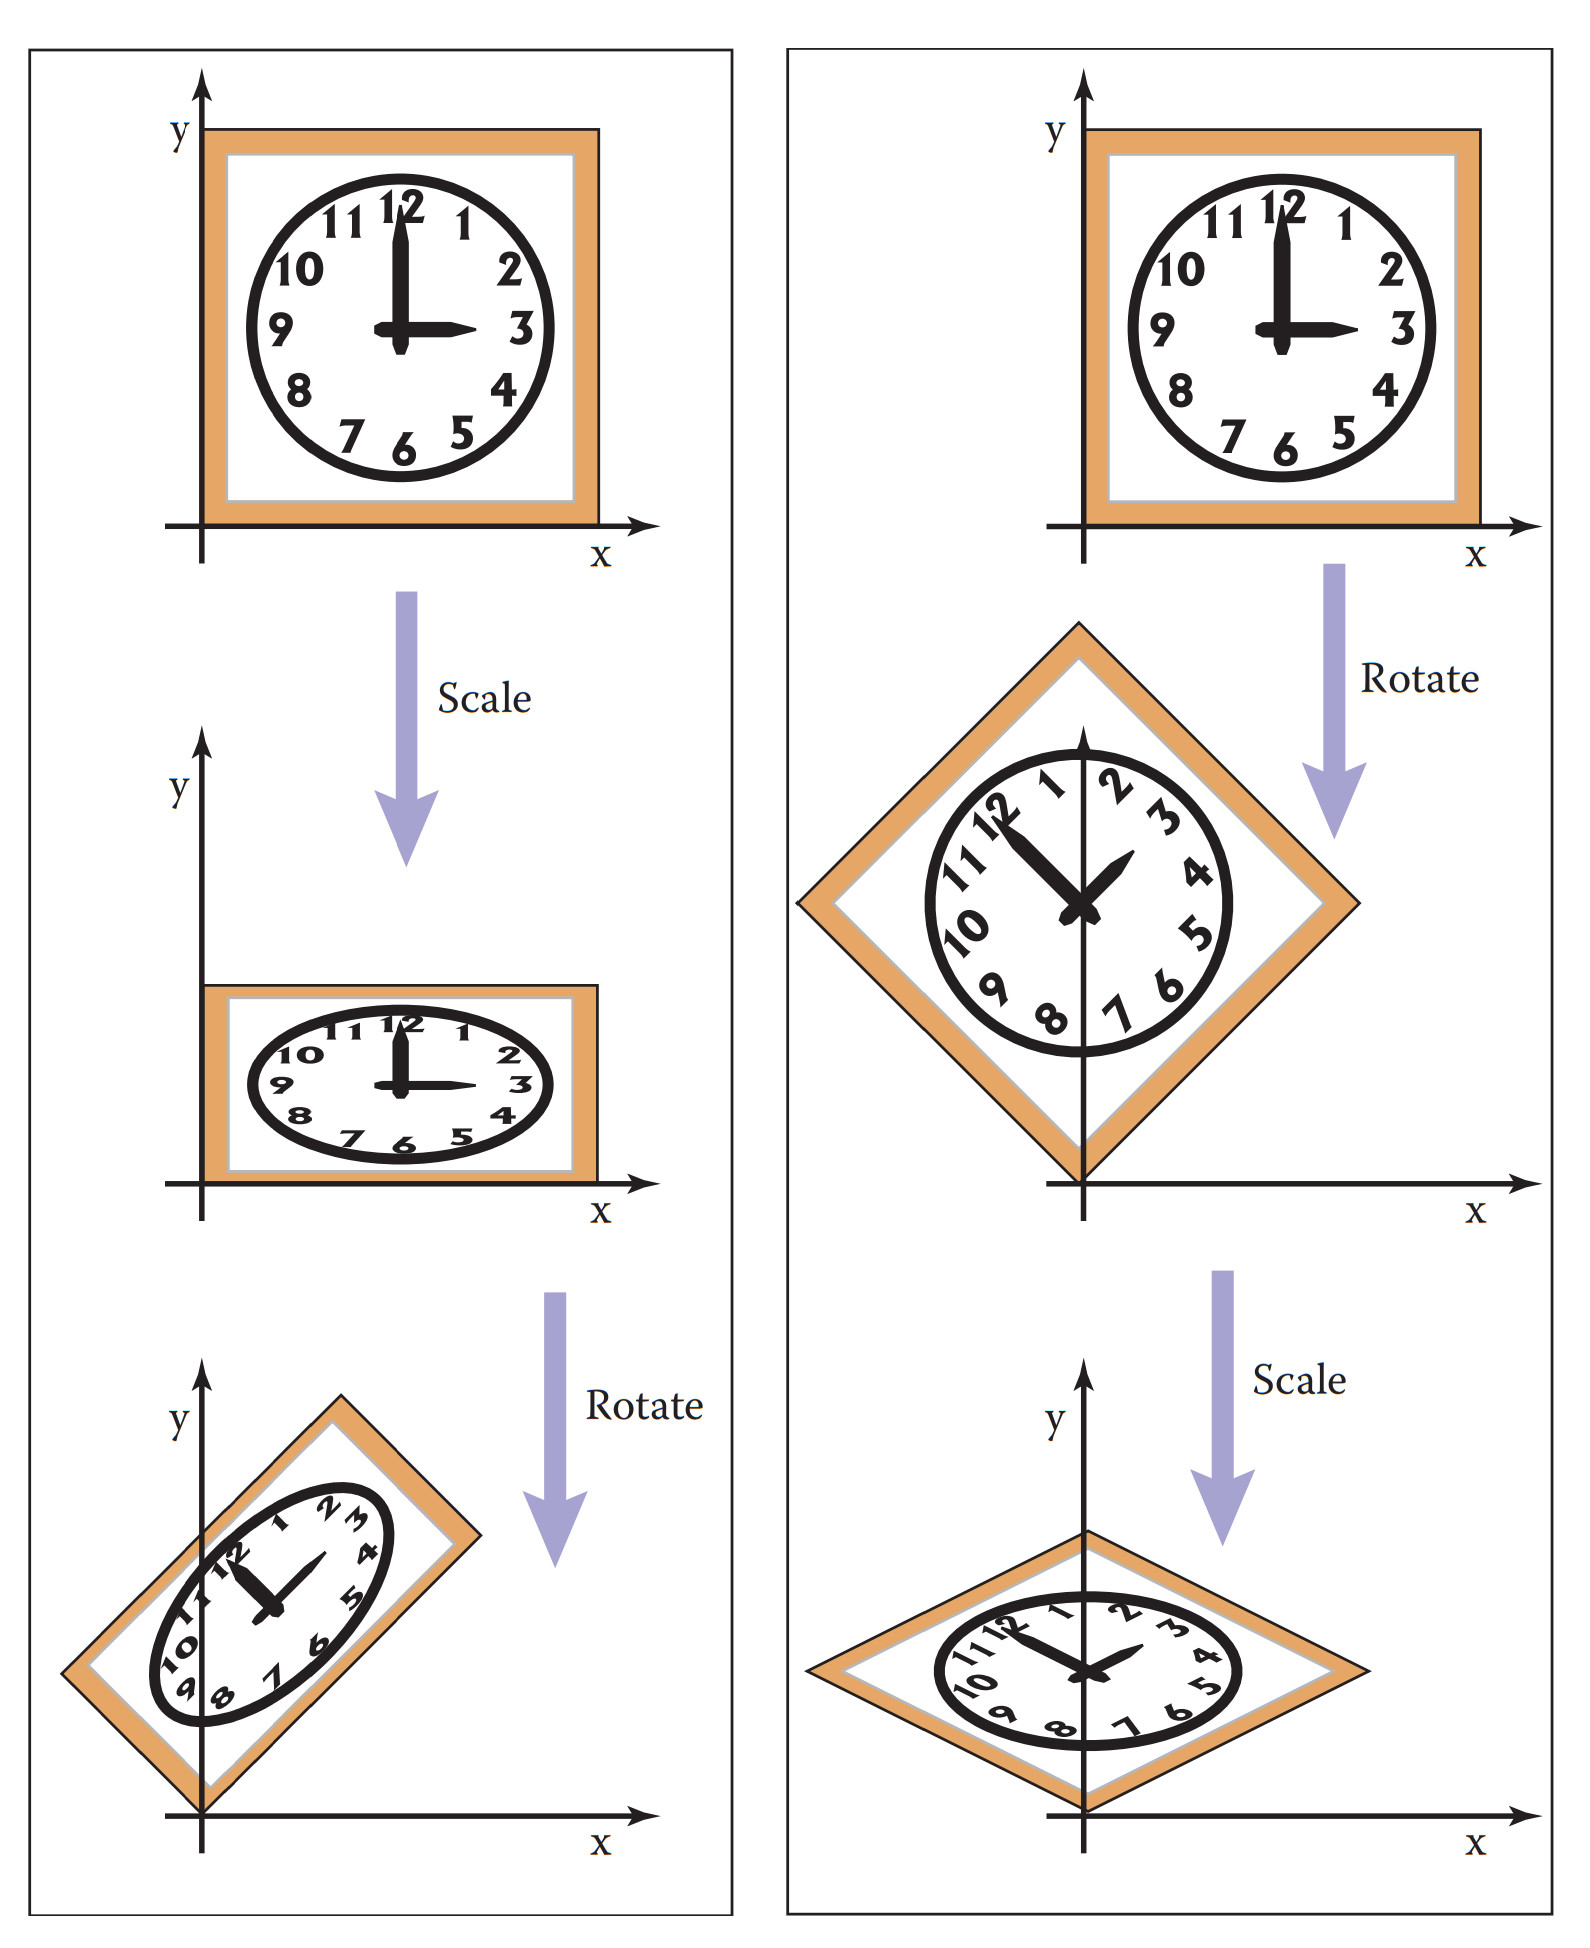
\includegraphics[scale=0.55]{Figure7.11.png}
	\caption{应用两种变换的顺序通常很重要。对于这个例子,我们在y轴上做了二分之一的缩放,然后旋转了$45^{\circ}$。将这两个变换的顺序颠倒一下,会产生不同的结果。}
	\label{fig:7.11}
\end{figure}	

\end{example}

\begin{example}
	使用我们提出的缩放矩阵,非均匀缩放只能沿坐标轴进行。
	
	
	
\end{example}

